\section{Automatic Image Processing}

In this section we provide detailed hands-on instruction on automatic image processing within 2dx \cite{scherer20142dx_automator}, including on-the-fly image drift-correction. The here described pipeline is optimised for data recorded on a direct electron detector, such as the Gatan K2 summit. 

\subsection{Real-time motion-correction}

In case you record dose fractioned movies we propose the drift-correct them on-the-fly as described in:

\textit{https://github.com/C-CINA/2dx/wiki/Automatic-Drift-Correction-C-CINA-setup}

Additionally instruction about setting up our automatic drift-correction pipeline is available under:

\textit{https://github.com/C-CINA/2dx/wiki/Automated-Drift-Correction-GUI}

2dx\_automator will later be used to automatically process the drift-corrected average of all frames.

\subsection{Required software}

2dx\_automator is only supported under Linux right now.
Please make sure that the list of dependencies is installed on the used system.

\begin{itemize}
	\item \texttt{TkInter} a python GUI package
	\item \texttt{py-thread} to be able to dispatch processing into different tasks
	\item \texttt{py-imaging (aka PIL)} the python image processing libraries
	\item \texttt{eman2/sparx} has to be installed and sourced on the system
	\item \texttt{py-matplotlib} to generate plots
	\item \texttt{py-shutil} for low-level operating system interaction
	\item \texttt{ImageMagic} especially the command-line tool \texttt{convert} has to be available
\end{itemize}

Additionally 2dx\_automator requires that \texttt{2dx\_image, 2dx\_merge} are available in the command line. If you installed a pre-compiled package please add 2dx's binary directory to your path:

\texttt{export PATH = /opt/2dx/bin:\$PATH}

If you compiled the software from source directly on your computer you should source the installation-binary folder as well:

\texttt{export PATH = <your\_install\_dir>/bin:\$PATH}

where \texttt{<your\_install\_dir>} equals the second argument passed to the \texttt{build\_all}-script. If you did not pass any argument to the build-script then \texttt{<your\_install\_dir>} equals \texttt{\textasciitilde{}/2dx/}.

\subsection{Automation setup}

The basic folder organisation is shown in \autoref{fig:autoworkflow}: The raw images are stored in the \textit{raw data folder}. Note that we here only process averages gained from drift-corrected movie-frames. 2dx\_automator will check for newly added images in this folder periodically (every second). In case a new image is added, this image is processed automatically with 2dx\_image: Defocus determination, lattice estimation, unbending, automatic masking, CTF-correction and map generation. Thereby the image is imported into the currently selected 2dx-project. This project contains a merge directory and a folder storing image-folders for each automatically processed image.

\begin{figure}
	\centering
	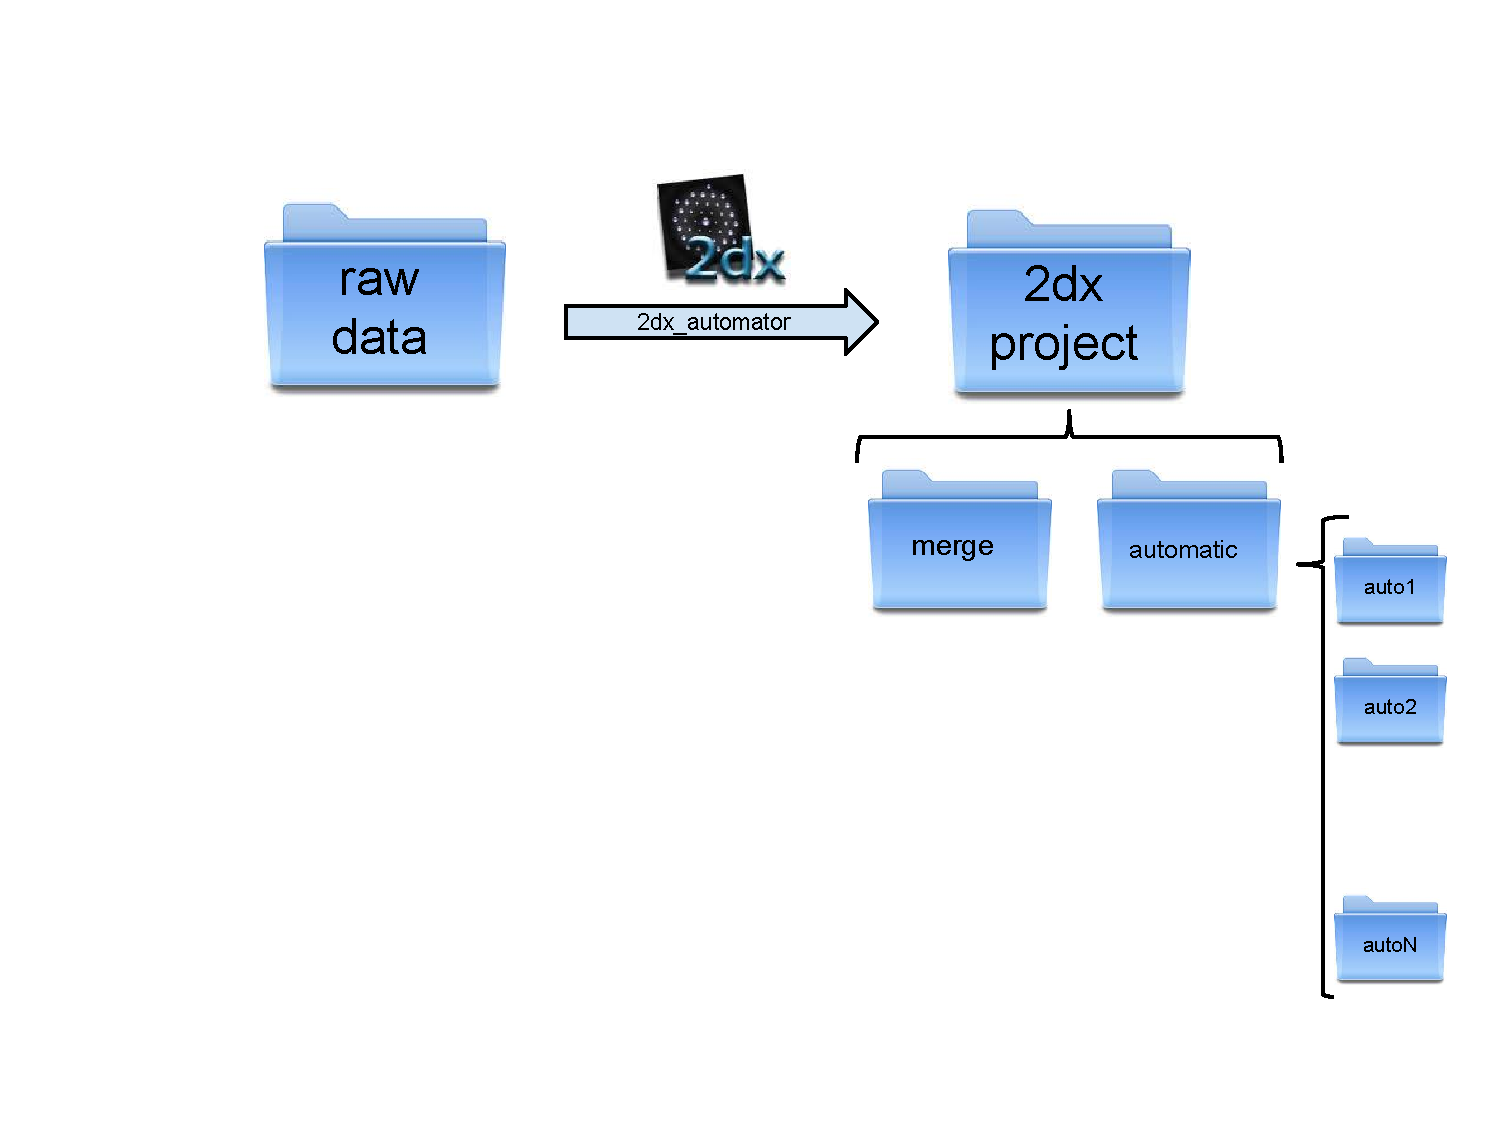
\includegraphics[width=1.0\textwidth]{auto_workflow.pdf}
	\caption{2dx\_automator: Folder structure}
	\label{fig:autoworkflow}
\end{figure}

Before launching the automation for the first time, create an empty folder, which will later contain your automatically populated 2dx-project. Then launch 2dx\_merge and select this newly generated folder as your project directory. 2dx\_merge asks whether the project structure should be generated, which should be done of course. Note that this step is only required when generating a new project. It is very important that the project structure is generated by 2dx\_merge before you launch the automation.

Starting the automation software is done by executing the command \texttt{2dx\_automator} in the shell. Given you installed all dependencies properly, 2dx\_automator will ask for two different folders. The first one you have to select is the raw images folder. Please note that you have to navigate into the folder before pressing \textit{"Ok"}, just selecting the desired folder does not work. Secondly you are asked to select the 2dx-project. Please select the root of the project, i.e. the \textit{2dx project} in \autoref{fig:autoworkflow}.

2dx\_automator requires a config-file that stores the processing parameters used for image processing of all image. The automation software uses the file \textit{2dx\_merge.cfg} in the merge directory of the project folder (More precisely: the file linked in \textit{2dx\_master.cfg} from the root level is used). We suggest that you determine the optimal processing parameters in 2dx\_merge by manually importing and processing one or a couple of images before launching automatic processing. Once you found the optimal processing parameters by manually processing an image in 2dx\_image you can use the tuned set of parameters as default via \textit{"File > Save as Project Default"}. Alternatively - in case you already have a valid file from a previous similar project - you can load a config file in 2dx\_automator via \textit{"Configuration > Load config from file"}.

Once you loaded or generated an optimal config-file, the  automatic processing is finally launched by clicking on the \textit{Launch automation} button (top-right). Note that in case there are so far unprocessed images in the input folder, these images will be processed first.


\subsection{2dx\_automator}

asdf  \autoref{fig:auto} adf.

\begin{figure}
	\centering
	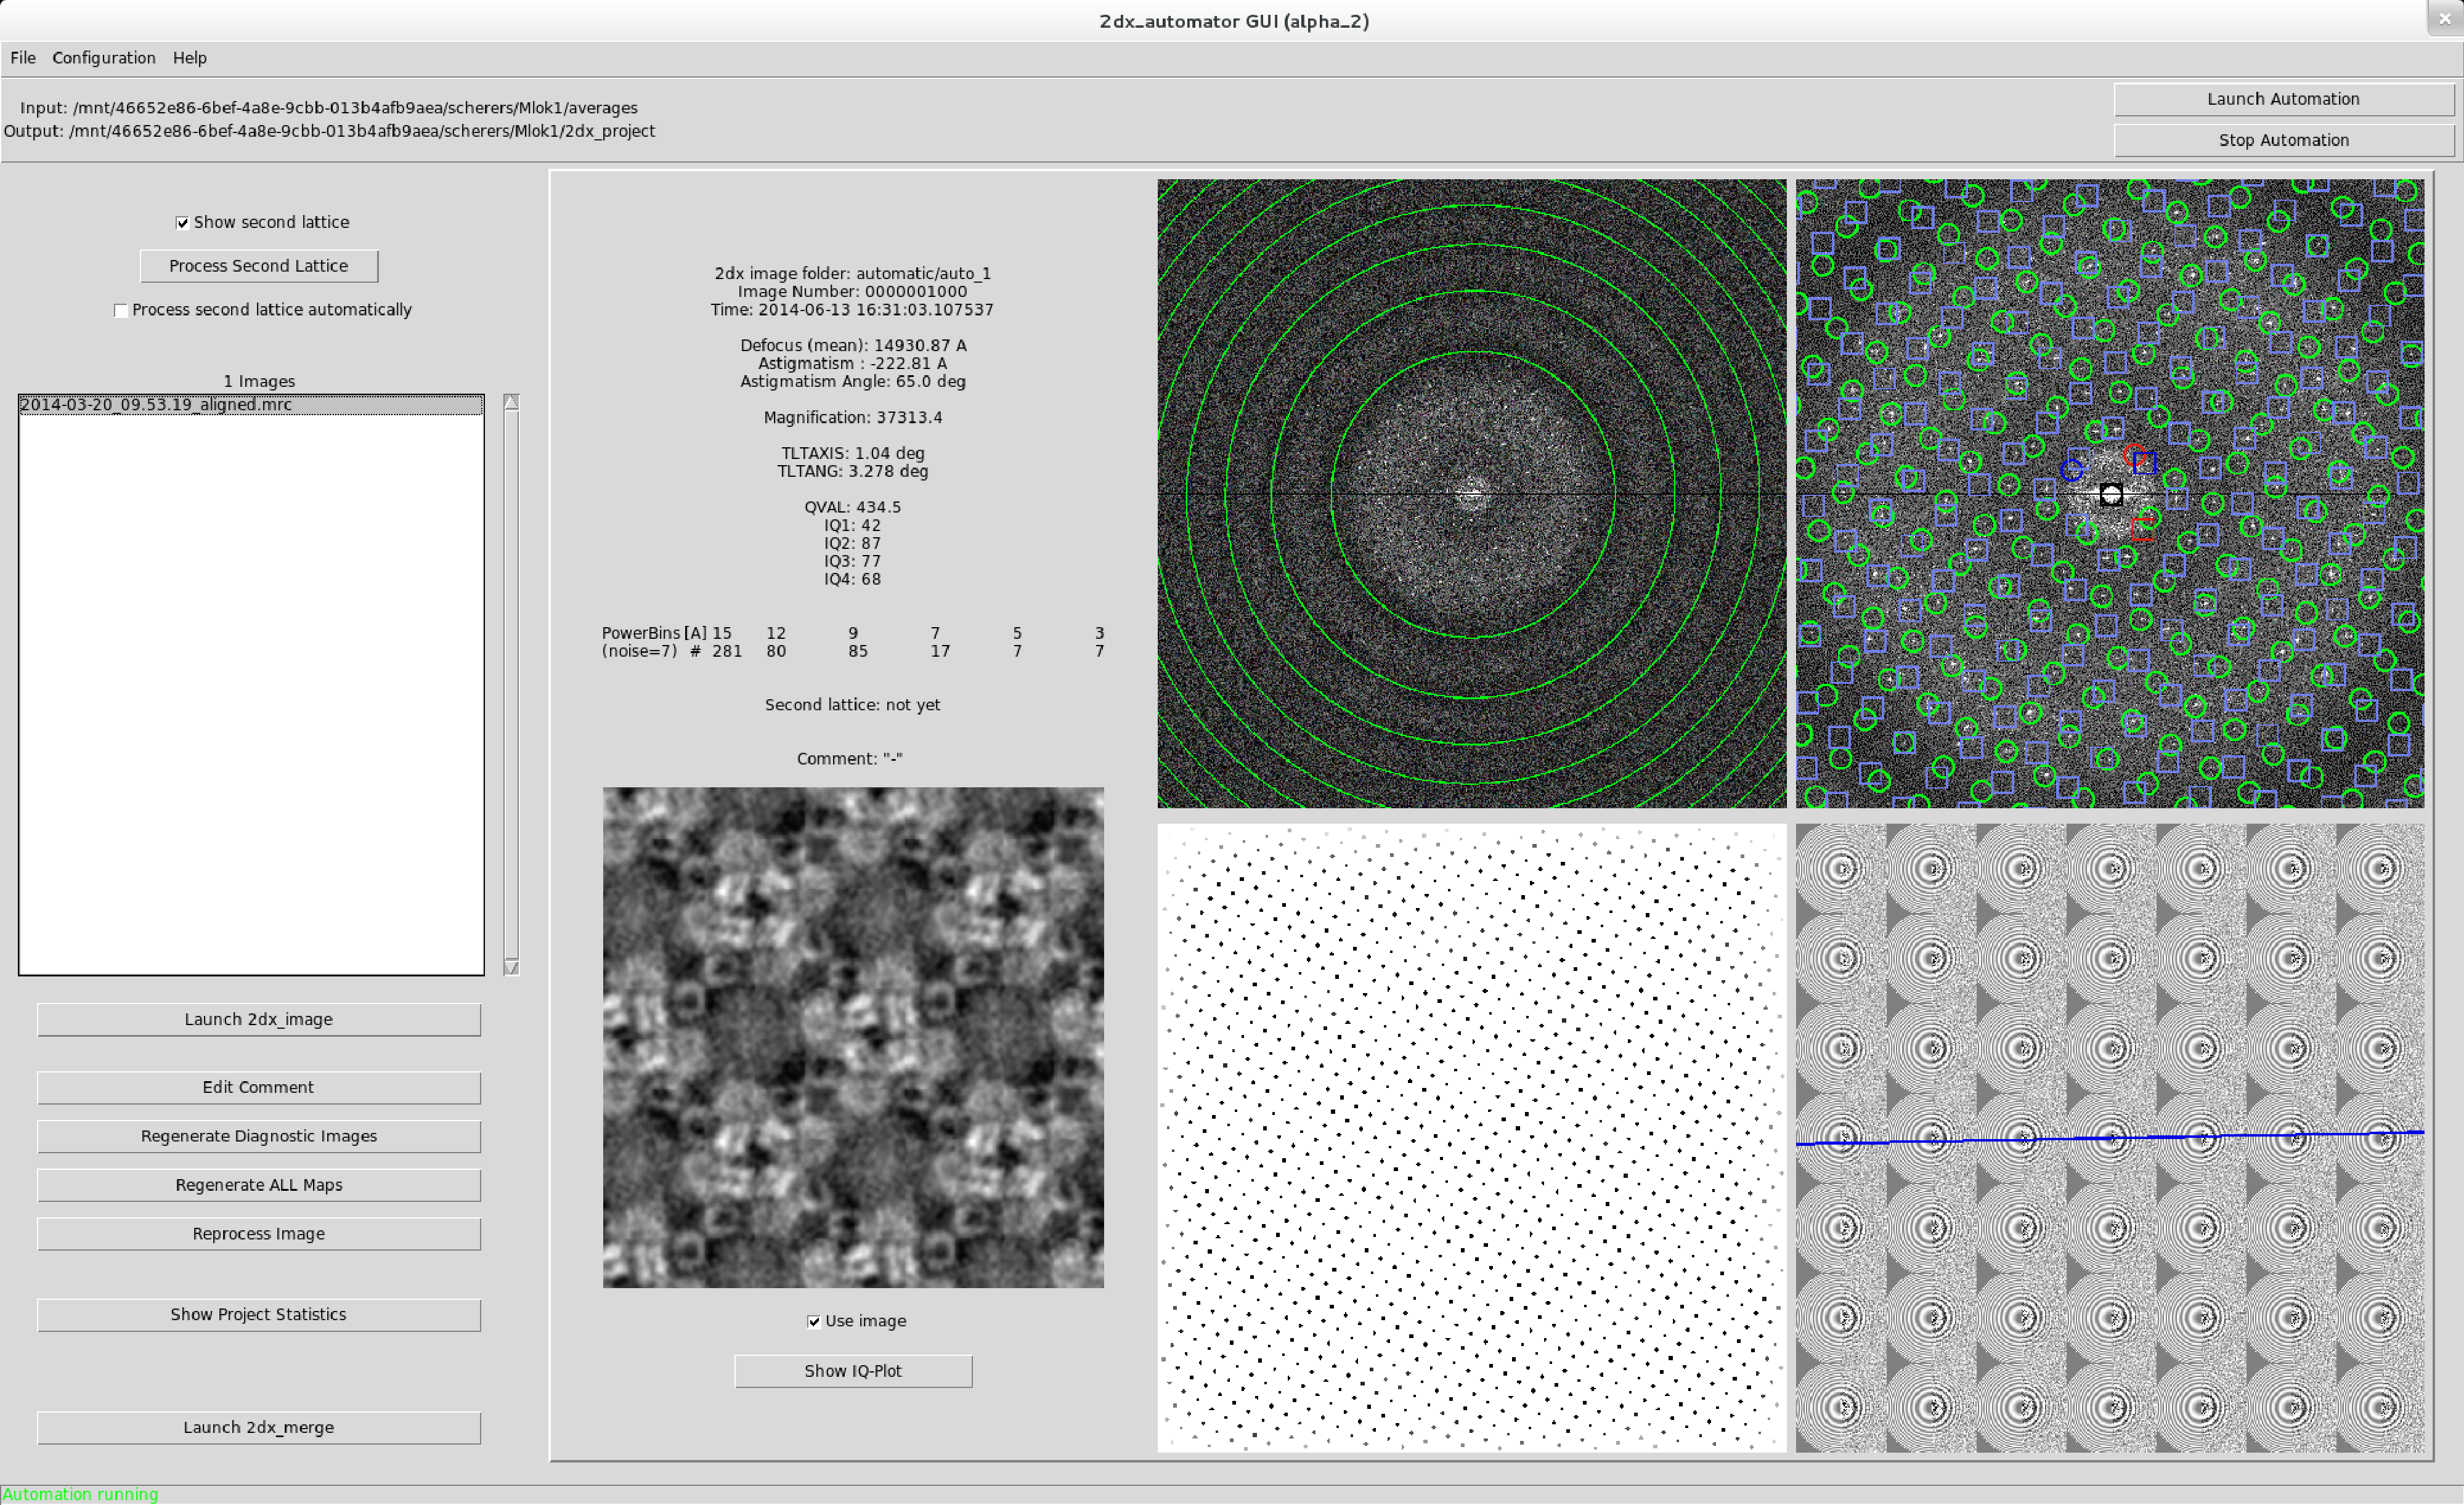
\includegraphics[width=1.0\textwidth]{auto.pdf}
	\caption{2dx\_automator}
	\label{fig:auto}
\end{figure}

\begin{figure}
	\centering
	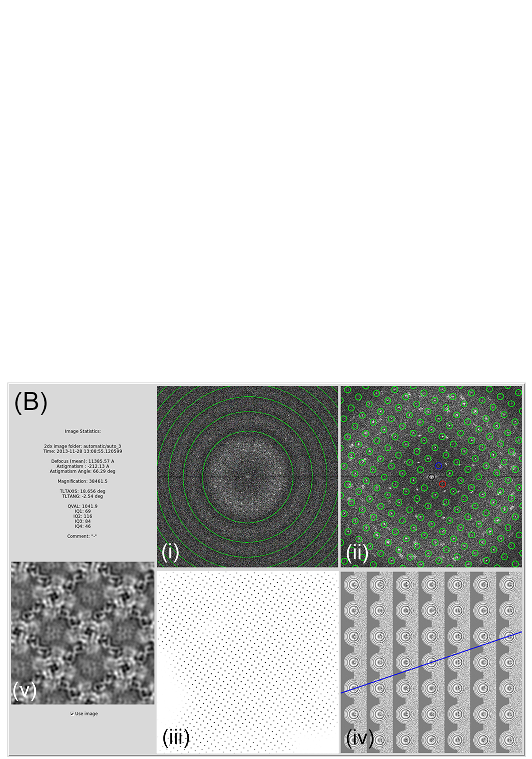
\includegraphics[width=1.0\textwidth]{auto2.pdf}
	\caption{Diagnostic view of the 2dx\_automator GUI. (i) Fourier transform with Thon rings and (ii) fitted lattice, (iii) peak profile from the unbending step used to mask the image, (iv) locally estimated defocus values, (v) final 2D projection map.}
	\label{fig:auto2}
\end{figure}


\subsection{Advanced tricks}

\begin{description}
	\item [Second lattice processing]
	\item [Manual processing intervention] 
	\item [Comment editing]
	\item [Updating image maps]
	\item [Reprocess an image]
	\item [Project statistics]
	\item [IQ-Stat analysis]
	\item [Configuration file handling] 
\end{description}



\begin{figure}
	\centering
	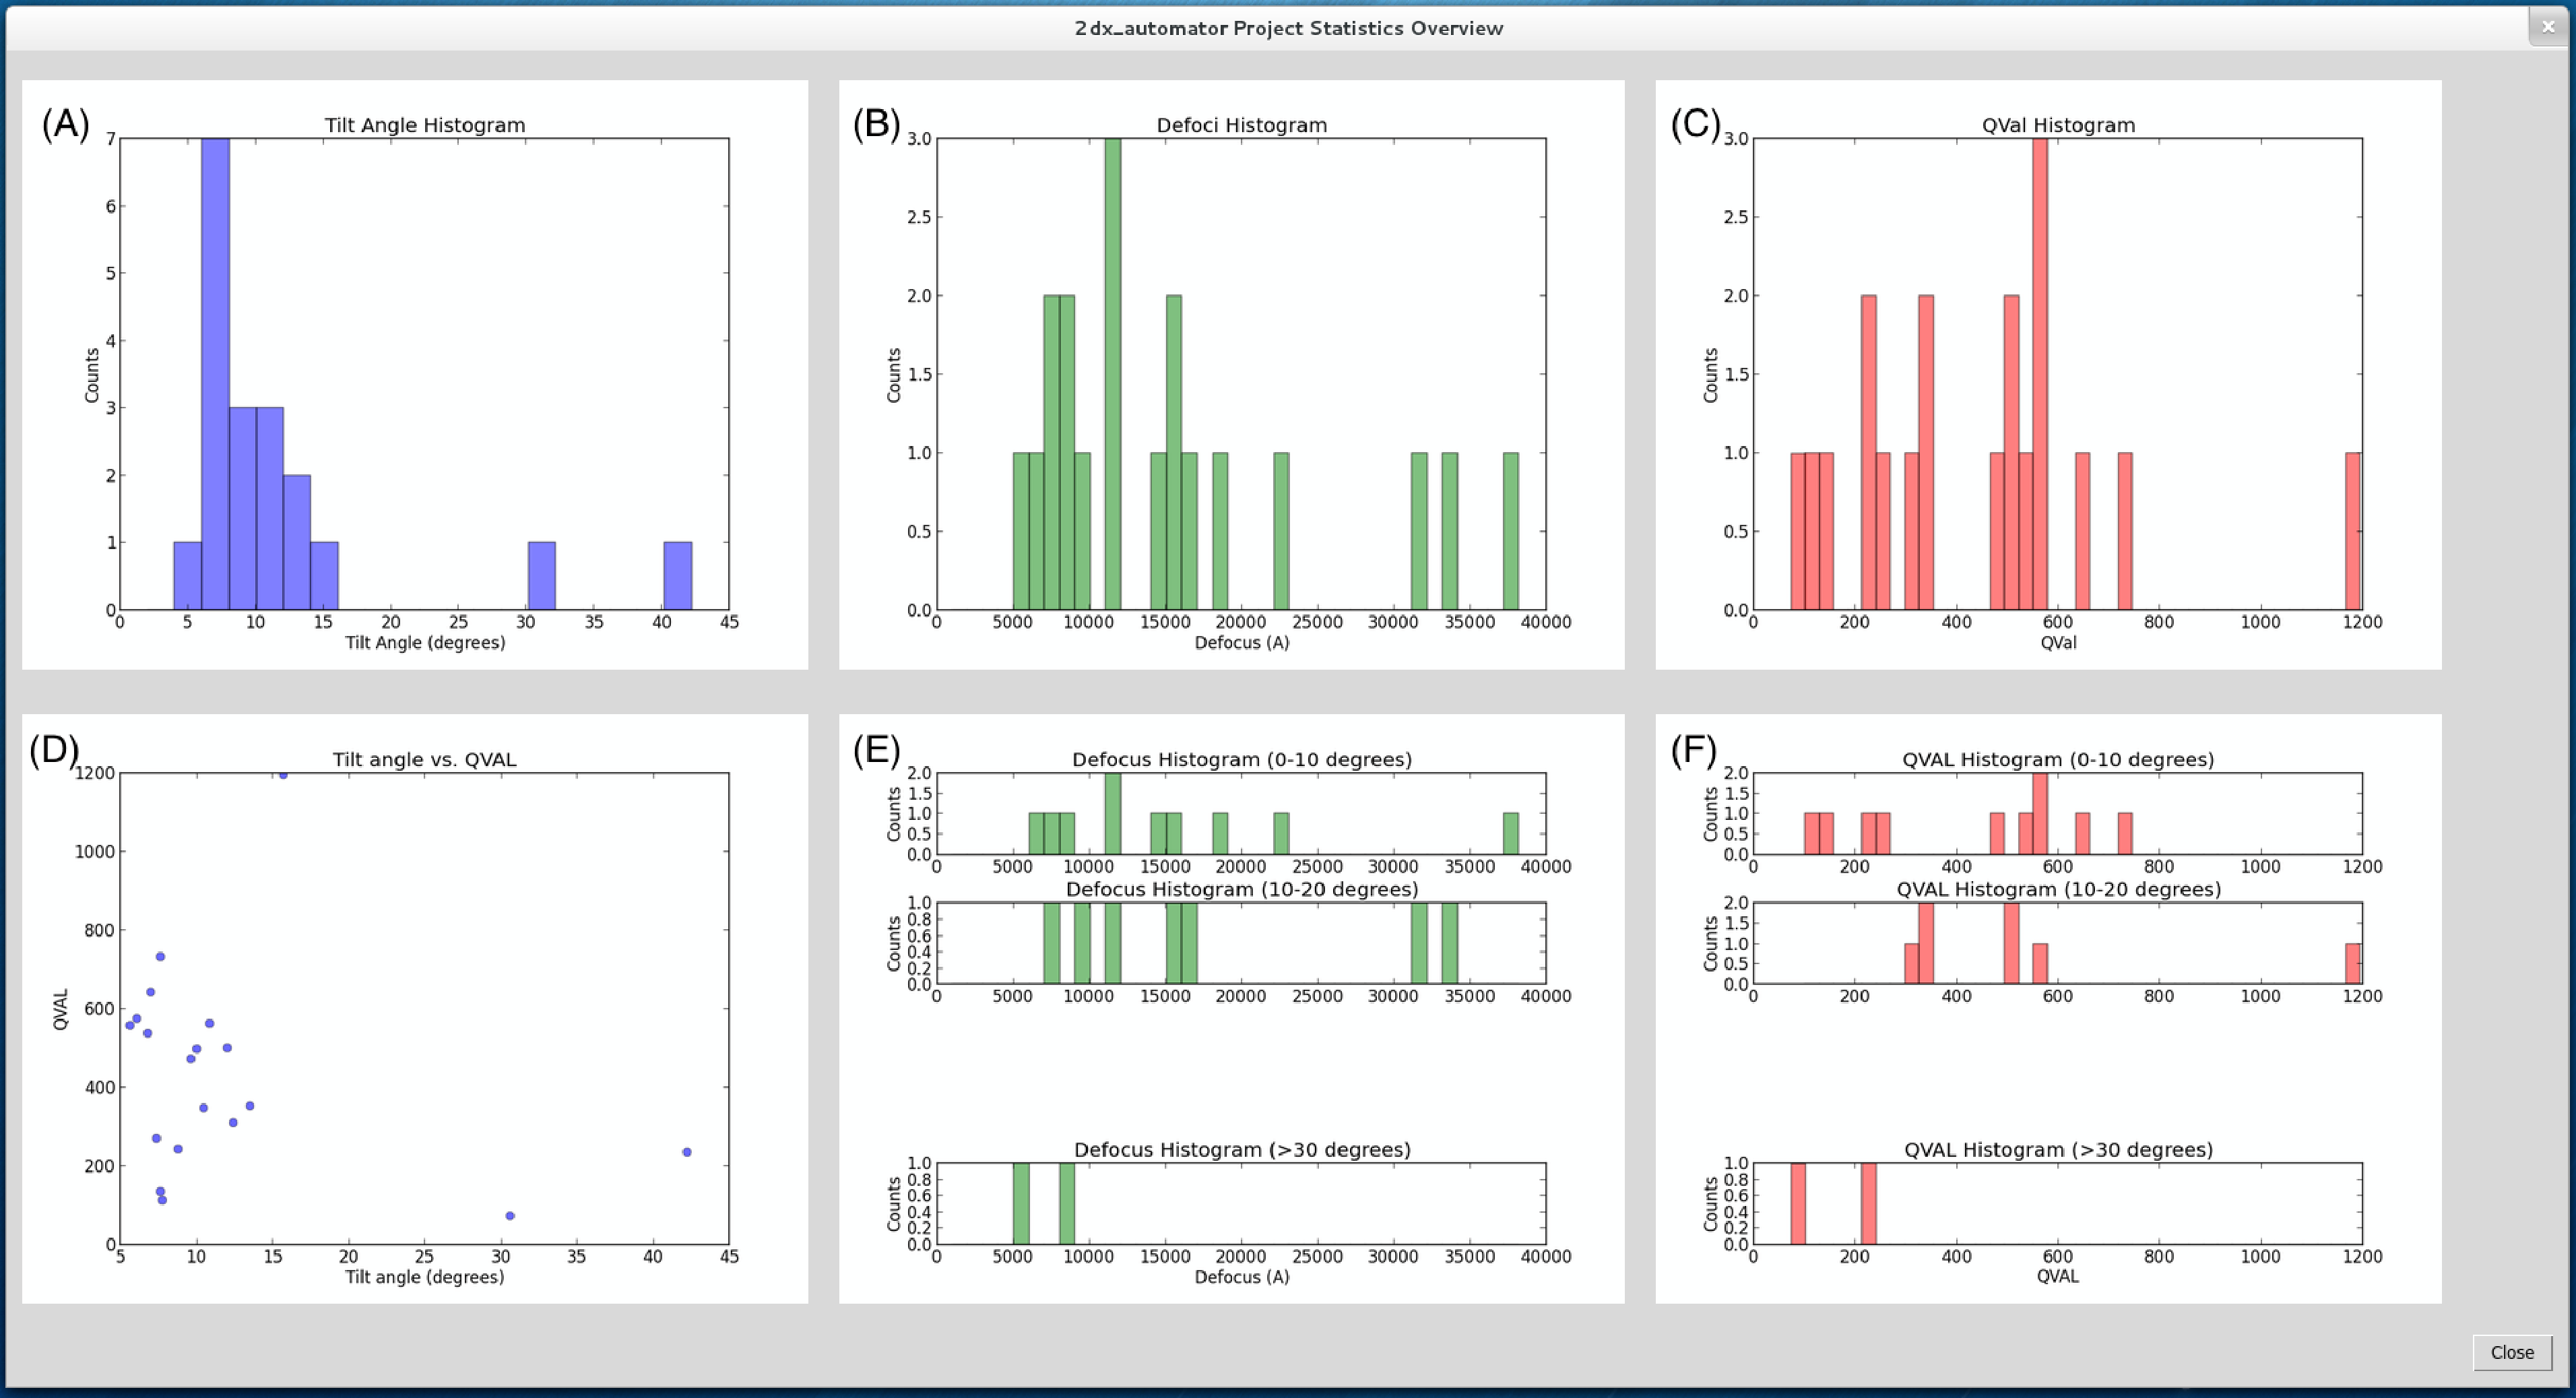
\includegraphics[width=1.0\textwidth]{auto_overview.pdf}
	\caption{Project stat}
	\label{fig:auto_stat}
\end{figure}